\documentclass{article}
\usepackage[utf8]{inputenc} %кодировка
\usepackage[T2A]{fontenc}
\usepackage[english,russian]{babel} %русификатор 
\usepackage{mathtools} %библиотека матеши
\usepackage[left=1cm,right=1cm,top=2cm,bottom=2cm,bindingoffset=0cm]{geometry} %изменение отступов на листе
\usepackage{amsmath}
\usepackage{graphicx} %библиотека для графики и картинок
\graphicspath{}
\DeclareGraphicsExtensions{.pdf,.png,.jpg}
\usepackage{subcaption}
\usepackage{pgfplots}
\usepackage{array}
\usepackage{pgfplots}
\pgfplotsset{compat=1.16}

\begin{document}
% НАЧАЛО ТИТУЛЬНОГО ЛИСТА
\begin{center}
    \Large
    Федеральное государственное автономное \\
    образовательное учреждение высшего образования \\ 
    «Научно-образовательная корпорация ИТМО»\\
    \vspace{0.5cm}
    \large
    Факультет программной инженерии и компьютерной техники \\
    Направление подготовки 09.03.04 Программная инженерия \\
    \vspace{1cm}
    \Large
    \textbf{Отчёт по лабораторной работе №2} \\
    По дисциплине «Математическая статистика» (четвёртый семестр)\\
    Исследование распределения случайной величины\\
    \large
    \vspace{8cm}

    \begin{minipage}{.33\textwidth}
    \end{minipage}
    \hfill
    \begin{minipage}{.4\textwidth}
    
        \textbf{Студент}: \vspace{.1cm} \\
        \ Дениченко Александр\\
        \ Разинкин Александр\\
        \ Соколов Анатолий\\
        \textbf{Практик}:  \\
        \ Милованович Екатерина Воиславовна
    \end{minipage}
    \vfill
Санкт-Петербург\\ 2024 г.
\end{center}
\thispagestyle{empty}

% КОНЕЦ ТИТУЛЬНОГО ЛИСТА 
\newpage
\section*{Цель работы}
Цель данной работы состоит в том, чтобы на основании опытных данных, используя метод моментов, построить оценки параметров законов распределения и оценки функции респределения и плотности вероятности.
\section*{Данные }
Закон: равномерный закон распределения\\
Выборка: 1.85 3.91 6.13 2.17 4.05 2.83 6.97 2.17 4.27 3.00 5.53 4.54 4.64 6.29 2.93 4.72 3.41 7.31 3.13
\section{Вариационный ряд}
1.85 2.17 2.17 2.83 2.93 3.00 3.13 3.41 3.91 4.05 4.27 4.54 4.64 4.72 5.53 6.13 6.29 6.97 7.31
\section{Точечная оценка математического ожидания}
\[\overline{m} = \frac{1}{n}\sum_{i=1}^{n}x_i \approx 4.20\]
\[\overline{\sigma}^2 = \frac{1}{n-1}\sum_{i=1}^{n}(x_i-\overline{m})^2 \approx 2.69\]
\section{Построение оценки}
Используя метод метод моментов, построим оценки параметров равномерного закона распределения, где равномерный закон распределения имеет следующий вид:
\\ \\
Случайная величина имеет непрерывное равномерное распределение на отрезке [a, b], если её плотность имеет вид:
\[f(x) = 
\begin{cases}
    0,\ x<a\\
    \frac{1}{b-a},\ a\leq x\leq b\ ;\\
    0,\ x>b
\end{cases}
 \] 
Функция распределения:
 \[F(x) = 
\begin{cases}
    0,\ x<a\\
    \frac{x-a}{b-a},\ a\leq x\leq b\ ;\\
    1,\ x>b
\end{cases}
\]
\section{Метод моментов}
Выразим числовые параметры теоретического распределения через моменты распределения, оценненные по выборки. 
Число моментов соответствовует числу неизвестных параметров распределения - 2.
\\Начальный момент для непрерывных случайних величин.
\[
    \nu_k = \int_{-\infty}^{\infty}x^kf(x)dx
\]
\[
    m = \int_{-\infty}^{\infty}xf(x)dx = \int_{-\infty}^{a} 0 dx +\int_{a}^{b}\frac{x}{b-a}dx + \int_{b}^{\infty}0dx = \frac{1}{b-a}\cdot \frac{x^2}{2}\biggr\rvert_a^b = \frac{b^2-a^2}{2(b-a)} = \frac{a+b}{2}
\]
Центральный момент:
\[\mu_k = M((x-m)^k) = \int_{-\infty}^{\infty}(x-m)^kf(x)dx\]
\[\sigma^2 = \int_{-\infty}^{\infty}(x-m)^2f(x)dx = \int_{-\infty}^{\infty}(x^2-2xm+m^2)f(x)dx = \int_{-\infty}^{a}0dx + \int_{a}^{b}x^2\cdot \frac{1}{b-a}dx - 2m\int_{a}^{b}x\cdot \frac{1}{b-a}dx +m^2\cdot \frac{1}{b-a}\cdot \int_{a}^{b}dx +\int_{b}^{\infty}0dx = \]
\[ = \frac{1}{b-a}\left(\frac{x^3}{3}\biggr\rvert_a^b-mx^2\biggr\rvert_a^b+\frac{m^2}{b-a}x\biggr\rvert_a^b\right) = \frac{1}{b-a}\left(\frac{b^3-a^3}{3}-m(b^2-a^2)+m^2\right)=\]
\[ = \frac{1}{b-a}\left(\frac{b^3-a^3}{3}-\frac{(a+b)(b^2-a^2)}{2}+\frac{(a+b)^2}{4}\right)= \frac{1}{b-a}\left(\frac{(b-a)(b^2+ab+a^2)}{3}-\frac{(a+b)^2(b-a)}{2}+\frac{(a+b)^2}{4}\right)=\]
\[= \frac{4(a^2+ab+b^2)-6(a+b)^2+3(a+b)^2}{12}= \frac{4a^2+4ab+4b^2-3a^2-6ab-3b^2}{12}=\frac{a^2-2ab+b^2}{12}=\frac{(b-a)^2}{12}\]
Получим:\\
\[
    \begin{cases}
        m = \frac{a+b}{2}\\
        \sigma^2 = \frac{(b-a)^2}{12}
    \end{cases} =>\ 
    \begin{cases}
        a+b = 2m\\
        (b-a)^2 = 12\sigma^2
    \end{cases} =>\ 
    \begin{cases}
        a+b = 2m\\
        b-a = 2\sqrt{3}\sigma
    \end{cases}
\]
\[a = 2m - b\]
\[b -(2m-b) = 2\sqrt{3}\sigma\]
\[2b - 2m = 2\sqrt{3}\sigma\]
\[b = m+\sqrt{3}\sigma\]
\[
    \begin{cases}
        a = m - \sqrt{3}\sigma\\
        b = m+\sqrt{3}\sigma
    \end{cases}
\]
Подставим a, b:
\[f(x) = 
\begin{cases}
    0,\ x<a\\
    \frac{1}{2\sqrt{3}\sigma},\ a\leq x\leq b\ ;\\
    0,\ x>b
\end{cases}
\] 
\[F(x) = 
\begin{cases}
    0,\ x<a\\
    \frac{x-m+\sqrt{3}\sigma}{2\sqrt{3}\sigma},\ a\leq x\leq b\ ;\\
    1,\ x>b
\end{cases}
\]
\\
Подставим $m, \sigma:$
\[f(x) = 
\begin{cases}
    0,\ x<1.36\\
    0.18,\ 1.36\leq x\leq 7.04\ ;\\
    0,\ x>7.04
\end{cases}
\] 
\[F(x) = 
\begin{cases}
    0,\ x<1.36\\
    0.18\cdot x- 0.24,\ 1.36\leq x\leq 7.04\ ;\\
    1,\ x>7.04
\end{cases}
\]
\newpage
\section{Построение оценок}
Построение графика плотности случайной величины:\\
\begin{center}
    \begin{tikzpicture}
        \begin{axis}[
            axis lines = middle,
            xlabel = \(x\),
            ylabel = {\(f(x)\)},
            xtick={1.36,7.04},
            ytick={0,0.18},
            yticklabels={0,0.18},
            xticklabels={1.36,7.04},
            ymin=0, ymax=0.25,
            xmin=0, xmax=8,
            every axis x label/.style={at={(ticklabel* cs:1.05)}, anchor=west,},
            every axis y label/.style={at={(ticklabel* cs:1.05)}, anchor=south,},
            legend pos=north west,
        ]
        
        % Функции
        \addplot[domain=0:1.36, samples=2, blue, line width=1mm] {0};
        \addplot[domain=1.36:7.04, samples=2, blue, line width=1mm] {0.18};
        \addplot[domain=7.04:8, samples=2, blue, line width=1mm] {0};
        
        % Вертикальные линии
        \draw [blue, line width=1mm] (axis cs:1.36,0) -- (axis cs:1.36,0.1825);
        \draw [blue, line width=1mm] (axis cs:7.04,0) -- (axis cs:7.04,0.1825);
        
        \addlegendentry{\(f(x)\)}
        
        \end{axis}
        \end{tikzpicture}
\end{center}
Построение графика функции распределения:\\
\begin{center}
    \begin{tikzpicture}
        \begin{axis}[
            axis lines = middle,
            xlabel = \(x\),
            ylabel = {\(F(x)\)},
            ymin=0, ymax=1.2,
            xmin=0, xmax=8,
            every axis x label/.style={at={(ticklabel* cs:1.05)}, anchor=west,},
            every axis y label/.style={at={(ticklabel* cs:1.05)}, anchor=south,},
            legend pos=north west,
            clip=false,
        ]
        
        % Функции
        \addplot[domain=0:1.36, samples=2, blue, line width=0.2mm] {0};
        \addplot[domain=1.36:7.04, samples=300, blue, line width=0.2mm] {0.18*x - 0.24};
        \addplot[domain=7.04:8, samples=2, blue, line width=0.2mm] {1};
        
        % Вертикальные линии для наглядности границ
        \draw [blue, line width=0.2mm] (axis cs:1.36,0) -- (axis cs:1.36,{0.18*1.36-0.24});
        \draw [blue, line width=0.2mm] (axis cs:7.04,{0.18*7.04-0.24}) -- (axis cs:7.04,1);
        
        \addlegendentry{\(F(x)\)}
        
        \end{axis}
        \end{tikzpicture}
\end{center}

\section*{Вывод}
На основании опытных данных нашли при помощи метода моментов параметры равномерного закона распределения, а также построили функцию распределения и плотность вероятности.
\end{document}
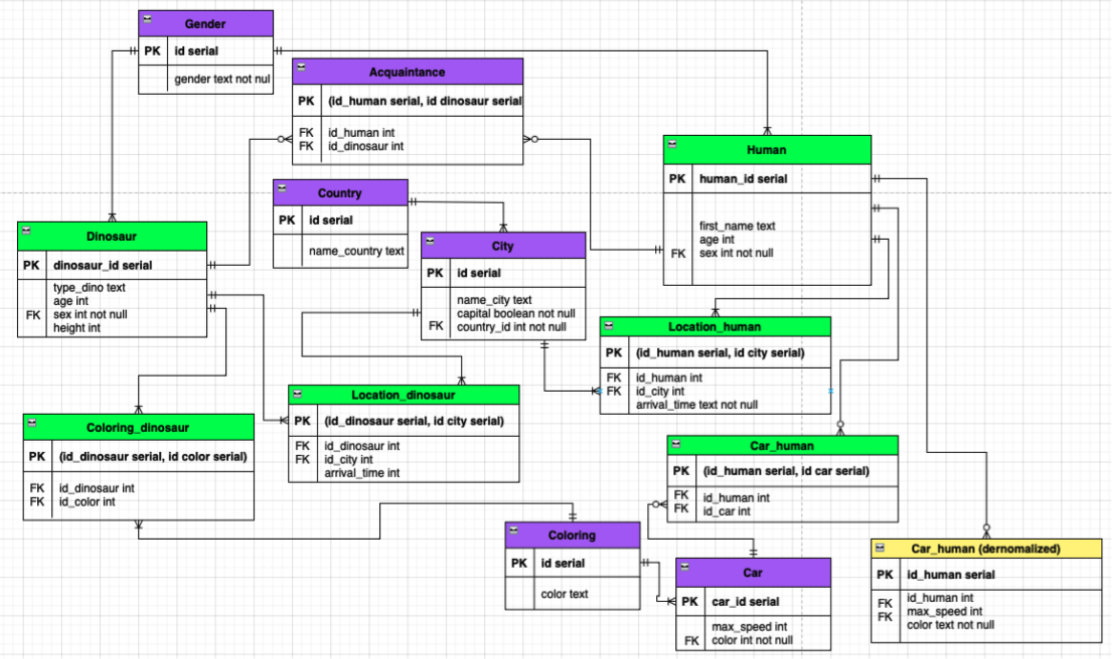
\includegraphics[width=.9\textwidth]{123}